\documentclass[a4paper, 12pt]{article}

\usepackage[T1]{fontenc}
\usepackage[utf8]{inputenc}
\usepackage[spanish, mexico]{babel}
\usepackage[style=mexican]{csquotes}
\usepackage[margin=2cm,top=2cm,includefoot]{geometry}
\usepackage[spanish, ruled, linesnumbered, lined]{algorithm2e}
\usepackage{amsmath, amsfonts, amssymb, amsthm, amsbsy, cancel}
\usepackage{microtype, parskip}
\usepackage{float, graphicx, subcaption}
\usepackage{circuitikz, tikz, pgfplots}
\usepackage{xcolor}
\usepackage{array, booktabs, multicol, multirow, tabularx}
\usepackage{hyperref, url}
\usepackage{siunitx}
\usepackage{tcolorbox}
\usepackage[style=ieee]{biblatex}
%definir el estilo de lapagina
\usepackage{fancyhdr}
%code
\usepackage{listings}


%variables de color
\definecolor{greenPortada}{HTML}{69A84F}
\definecolor{CabeceraAcero}{HTML}{5DADE2}
\definecolor{Cabeceraverde}{HTML}{008080}
\definecolor{CabeceraTomate}{HTML}{FF4500}



%cabecera
\setlength{\headheight}{40pt}
\pagestyle{fancy}
\fancyhf{}
\renewcommand{\headrulewidth}{3pt}
\renewcommand{\headrule}{\hbox to \headwidth{\color{Cabeceraverde}\leaders\hrule height \headrulewidth\hfill}}

%variables globales

\newcommand{\lineal}{img/lineal.png}
\newcommand{\nolineal}{img/nol.png}
% \newcommand{\}{img/}
% \newcommand{\}{img/}
% \newcommand{\}{img/}
% \newcommand{\}{img}

% \newcommand{\codeA}{code/}
% \newcommand{\codeB}{code/}


%gestion de hipervinculos
\hypersetup{
    breaklinks=true,
    colorlinks=true,
    citecolor=black,
    filecolor=magenta,
    linkcolor=black, 
    urlcolor=cyan
}
%gestor de codigo
\lstset{
    language=Matlab,
    basicstyle=\ttfamily,
    keywordstyle=\color{CabeceraAcero},
    commentstyle=\color{green!50!black},
    stringstyle=\color{CabeceraTomate},
    numbers=left,
    numberstyle=\tiny,
    numbersep=5pt,
    frame=single,
    breaklines=true,
    breakatwhitespace=true,
    tabsize=2
}

%Encabezado
\title{Redes convolucionales}
\author{Universidad Nacional Autónoma de México.\\Facultad de Estudios Superiores Cuatitlán.\\Palomino Alfonso Edgar.\\Vargas Gachuz Alonso}
\date{\today}
\cfoot{\thepage}

\begin{document}
    \maketitle 
    \begin{abstract}      
        El uso de las redes neuronales convolucionales \emph{(RNC)} se da a partir de un mejor manejo de imágenes a través de esta, que haciendo uso de redes neuronales con funciones lineales. Esto en conjunto con la capacidad de cómputo dispuesta en aumento, permiten su implementación, ya que a través de una tarjeta gráfica pequeña pero potente se pudo realizar el procesamiento de 4 imágenes que se etiquetaron pero no se trataron tomando en cuenta un conjunto de datos sin un tratamiento adecuado que si bien es posible encontrarlo en la realidad no es sencillo realizarlo, lo cual puede dificultar la implementación para un proyecto concreto donde, como este caso, se busca responder a casos específicos como señales de activación para un sistema. 
    \end{abstract} 
    \vspace{2ex}

    \section{Introducción.}
    El uso de redes neuronales de funciones lineales limitan las dimensiones o parámetros que se pueden trabajar en conjunto para el diseño de la red neuronal, ya que se busca segmentar la salida a un caso positivo o negativo sobre una línea recta como se puede observar en la figura~\ref{fig:lin}, cosa que se complica al tener más parámetros de entrada para el análisis, este caso se presenta en las imágenes al tener como entradas más de una dimensión para el análisis dejando un sistema mucho más complejo como en la figura~\ref{fig:nolin}, debido a esto es que se plantean las RNC que además de tener diferentes capas de entrada tiene la particularidad de usar redes simples que extraen características particulares cada una, las cuales pasan a otra neurona que agrupa dichas características para determinar un patrón más complejo sobre la imagen, de esta manera es que se pueden reconocer curvas y líneas en conjunto para determinar que algo es una mano o una manzana, este modelo está basado en el sistema de neuronas en la corteza visual primaria de un cerebro biológico. 
    El proceso de extracción de información resulta interesante debido a que en el caso más simple, el cual se representa por un arreglo unidimensional donde se puede extraer el valor de 0 y 1 a valores discretos en el intervalo de 0 a 255, (una escala de grises) se puede obtener un mapa de bits que representa sobre una imagen que valor de blanco o negro se puede obtener algo parecido a el sistema de control difuso, donde no se asigna un valor absoluto del sistema si no que se segmenta sobre una escala y en función de esto se considera una reacción, pero esto representa una limitante, independientemente del color, de que se tiene una posición absoluta del arreglo de bits a identificar, esto genera confusión a las salidas ya que si deslizamos, rotamos, o manipulamos la imagen de alguna manera, esta perderá la coincidencia con dicho mapa, esto como se comentó anteriormente se arregla colocando o centrando la atención de la red sobre patrones básicos (líneas, curvas, etc.) que forman o resultan indispensable sobre la imagen, lo cuales se agrupan para formar un mapa de coincidencia de dichas figuras, de esta manera no importa si el arreglo de bits no coincide, lo que importa es que ciertos patrones estén presente sobre la imagen, además de que a mayor detalle más nutre a la red cosa que sin las RNC no ocurre ya que tener más de una dimensión genera funciones indeterminadas sobre las cuales no se puede obtener una segmentación correcta de los casos donde la salidas son correctas o no, así de esta manera si el color no es indispensable ayuda a tener un patrón de figuras básicas que determina si algo es una manzana o un perro, si además de eso se le agrega los 3 parámetros de color para determinar si una figura redonda es una uva, un coco o un melón, la red es más precisa al tener más detalles, pero estop requiere un data de mayor tamaño, esto con el fin de adecuar la RNC para que funcione de la mejor manera. 


    \begin{figure}[H]
        \centering
        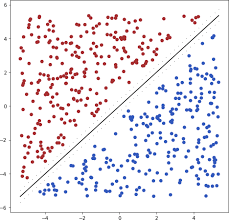
\includegraphics[width=0.4 \linewidth]{\lineal}
        \caption{Conjunto separable linealmente}
        \label{fig:lin}
    \end{figure}

    \begin{figure}[H]
        \centering
        \includegraphics[width=0.4 \linewidth]{\nolineal}
        \caption{Conjunto no separable de manera lineal}
        \label{fig:nolin}
    \end{figure}

    \section{Estado del arte.}

    

    %conocimientosP
    \section{Conocimientos previos.}
    El valor de las RNC está en procesar en paralelo las características de una imagen sin depender de la información que esta proporciona, si bien el orden de dichos valores es importante para el color ya que se utiliza un sistema RGB, el resto de la imagen depende más de la figuras propias del objeto que la RNC pueda identificar para determinara patrones claves que realizan la coincidencia de una imagen con su etiqueta.


    \subsection{Lógica difusa.}

    \subsection{Conjuntos borrosos}

    \subsection{Función de membresía}

    \subsection{Fuzzificación}

    \subsection{Mamdani.}

    \section{Metodología.}

    \section{Análisis de resultados.}

    \section{Conclusión}

\end{document}


    % \begin{equation}
    %     A = \{ ( x,\mu_{A(x)} )/x \in X \}
    % \end{equation}
    % Donde $\mu_{A(x)}$ es una función de pertenencia cuya etiqueta es A y su dominio es $x$
    .
    % \begin{figure}[H]
    %     \centering
    %     \includegraphics[width=0.8 \linewidth]{\conjuntoD}
    %     \caption{Conjuntos difusos}
    %     \label{fig:conjuntoD}
    % \end{figure}

    %\clearpage
    % \lstinputlisting[caption={Ejemplo de código MATLAB.}, label=lst:fis, title={ código 1 : Archivo del sistema de control difuso Mamdani}]{\codeB}

    % \begin{figure}[H]
    %     \centering
    %     \begin{subfigure}{0.8\linewidth}
    %         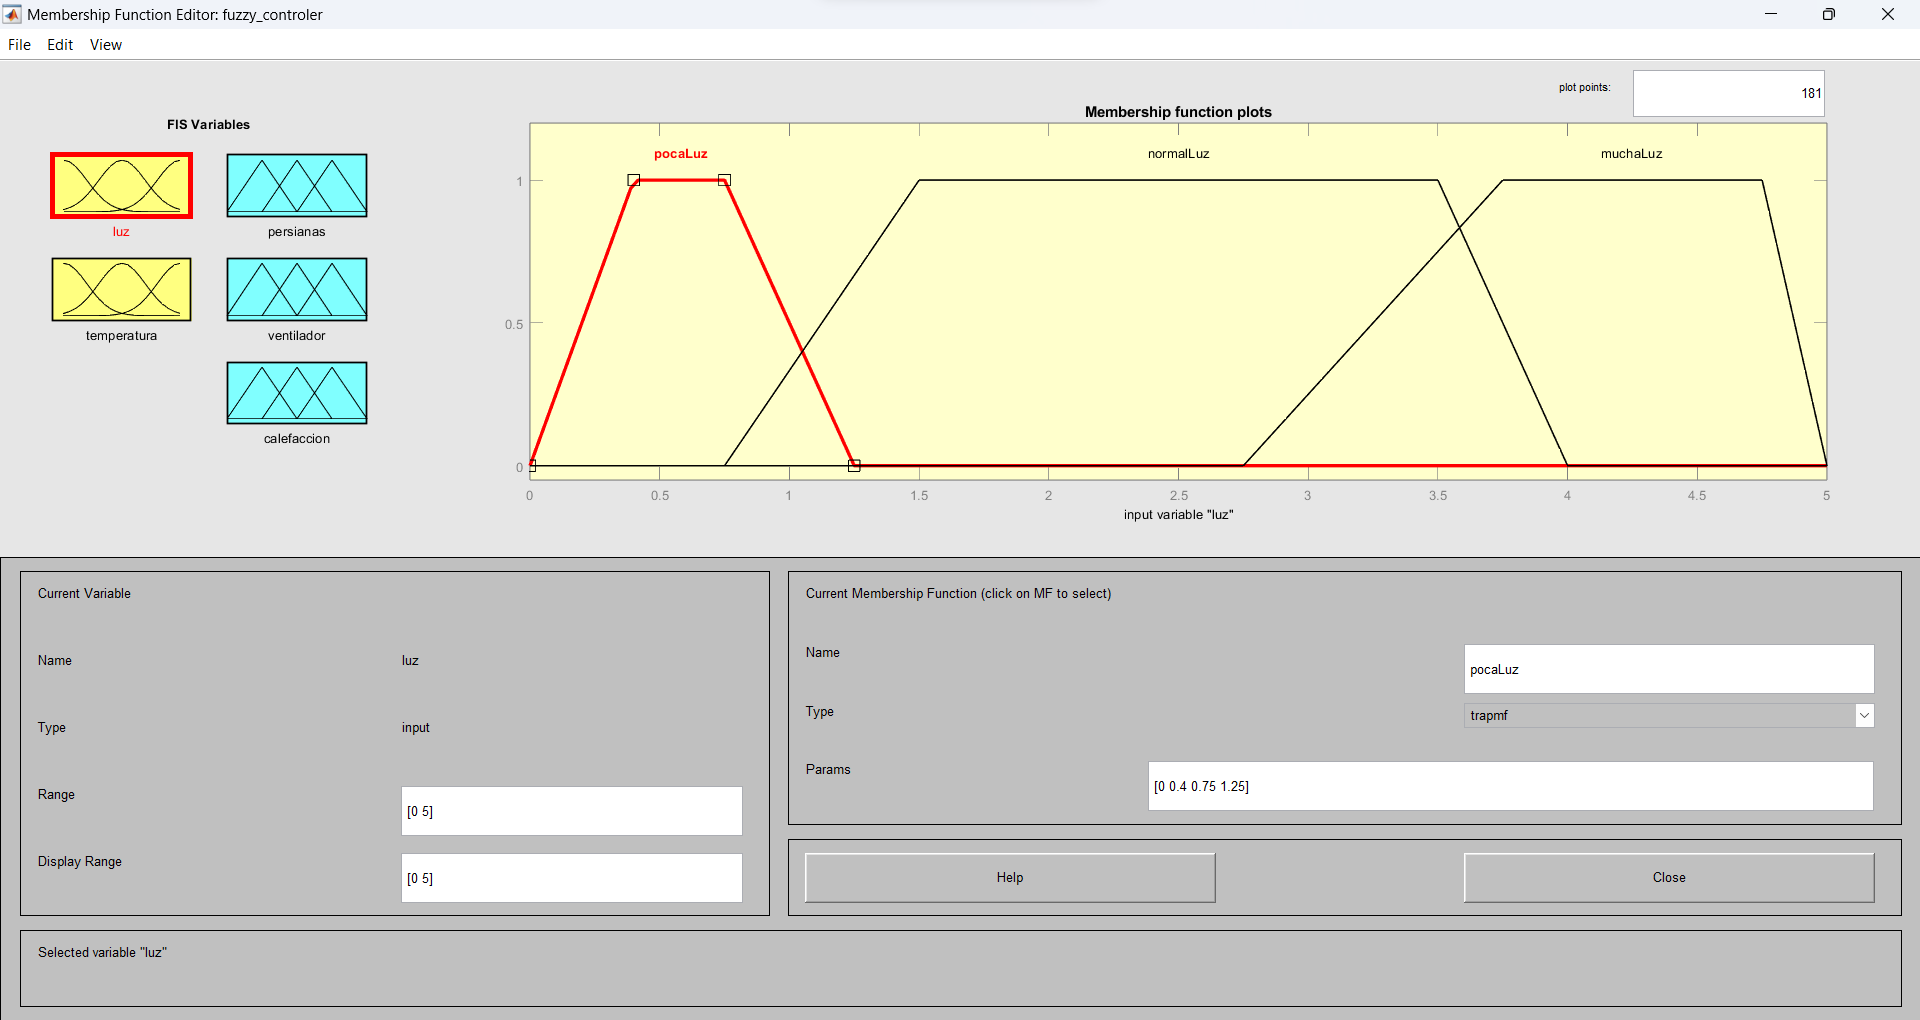
\includegraphics[width=\linewidth]{\luz}
    %         \caption{Conjunto difuso luz}
    %         \label{sub:luz}
    %     \end{subfigure}
    %     \begin{subfigure}{0.8\linewidth}
    %         \includegraphics[width=\linewidth]{\temperatura}
    %         \caption{Conjunto difuso temperatura}
    %         \label{sub:temp}
    %     \end{subfigure}
    %     \caption{Entradas}
    %     \label{fig:nter}
    % \end{figure}